\documentclass[letterpaper,journal]{IEEEtran}
\usepackage{amsmath,amssymb,amsfonts,array,booktabs,tabularx}
\usepackage{graphicx,xcolor,algorithm,algorithmic,tikz,cite,url}
\usepackage{microtype}
\usetikzlibrary{arrows.meta,positioning,fit}
\usepackage[hidelinks]{hyperref}
\hypersetup{pdftitle={FreqDuet: Cumulative Holding Budgets for Fixed-Fleet Timetable Coordination},pdfauthor={Anonymous Authors}}
\newcommand{\E}{\mathbb{E}}
\newcommand{\clip}{\operatorname{clip}}
\newcommand{\pos}[1]{[#1]_+}
\newcolumntype{Y}{>{\raggedright\arraybackslash}X}
\newcommand{\ManualBudgetGain}{2.396}
\newcommand{\ManualReadinessGain}{4.540}
\newcommand{\ManualBudgetCV}{+0.003025}
\newcommand{\LearnedBudgetGain}{1.645}
\newcommand{\HarmonicJourney}{-0.562}
\newcommand{\HarmonicCV}{-0.000937}
\newcommand{\PressureStaticGain}{3744.15}
\newcommand{\PressureCapGain}{3123.80}
\newcommand{\JointStaticLoss}{6.803}
\newcommand{\JointCapLoss}{10.744}

\hyphenation{time-table time-tables co-or-di-na-tion}
\begin{document}
\title{FreqDuet: Cumulative Holding Budgets for Fixed-Fleet Timetable Coordination}
\author{Anonymous Authors}
\markboth{RESEARCH DRAFT, NOVEMBER 2026}{Cumulative Holding Budgets and Vehicle Circulation}
\maketitle
\begin{abstract}
Terminal timetable revisions and en-route holding compete for the same vehicle time. We study their coordination through persistent trip-level holding budgets shared by forecasting, legal-action enumeration, and physical execution. The system combines causal demand summaries, a bounded timetable law, and a model-based fast controller; a learned publication-permission policy is evaluated separately. On 16 independent simulation demand days, reducing the manual joint controller's budget retention from 0.50 to 0.25 reduced restricted journey exposure by \ManualBudgetGain\ s/passenger and readiness delay by \ManualReadinessGain\ s/trip, while increasing actual headway CV$^2$ by \ManualBudgetCV. On another 16 new days, pressure-driven credit reduced public dispatch delay relative to development-exposure-matched static-credit and stop-cap mixtures, but both comparisons failed prespecified regularity protection. A further 144-path factorial supplement covered nominal, light, heavy and shifted-peak demand, with four new paired days per condition. Joint control reduced journey exposure by 6.84--27.56 s/passenger and readiness delay by 27.52--60.26 s/trip relative to fixed360 bilateral holding, again at increased actual CV$^2$. Conditional contrasts identified budgets as the main source of circulation savings; adding the timetable law did not consistently improve service. Matched-budget learning and the primary harmonic-journey comparison did not establish additional passenger gains. The evidence supports an executable vehicle-time interface and condition-dependent operational tradeoffs, not a general improvement over simple limits at preserved regularity.
\end{abstract}
\begin{IEEEkeywords}
Bus holding, timetable coordination, vehicle circulation, cumulative time budgets, model-based control, paired simulation.
\end{IEEEkeywords}
\section{Introduction}
\IEEEPARstart{H}{olding} a bus can improve service spacing while delaying the passengers already on board. Under a fixed fleet, the same seconds can also postpone the vehicle's next departure. A terminal timetable revision therefore depends not only on demand and the current terminal queue, but also on how much vehicle time downstream holding will consume. This study examines that connection through a shared cumulative holding budget.

The service--holding tradeoff is established in the bus-control literature. Daganzo's headway-based control seeks reliable high-frequency service with reduced schedule slack~\cite{daganzo2009headway}. Daganzo and Pilachowski extend cooperation to front and rear spacing, using speed adjustment to counter large gaps~\cite{daganzo2011cooperation}. Berrebi \emph{et al.} compare predictive and non-predictive holding methods in terms of headway stability and holding time~\cite{berrebi2018comparing}. These findings motivate a direct question: does a turnover-aware allocation rule improve the operating tradeoff relative to simple holding restrictions, or does it mainly choose a different point on that tradeoff?

An executable comparison requires consistent resource semantics. A timetable predictor can assume a returning vehicle will be available while later holding delays that return. A cumulative allowance can also have different effects from a per-stop cap even when both lead to similar average holding. We address these issues by using the same published releases, irreversible commands, and remaining-credit ledger inside each forecast and in physical execution. This makes a budget an inspectable resource constraint rather than an additional reward term.

The architecture also permits a controlled examination of temporal information and learning. Causal harmonic summaries inform a bounded timetable law; the fast layer evaluates legal holding actions on current automatic passenger count (APC) and automatic vehicle location (AVL) observations. A learned supervisor can enable or withhold timetable revisions, but the same interface can be driven by an always-joint manual supervisor. Matching their budget settings separates a learning increment from a change in holding exposure. Matching a harmonic and non-harmonic representation addresses a different question again.

We investigate three questions. First, how can published releases, cumulative holding permissions and irreversible commands refer to the same vehicle-time resource? Second, does changing that resource limit improve service, or primarily redistribute cost between passengers, regularity and subsequent trips? Third, which changes are attributable to timetable coordination, budget allocation or their interaction? The contribution is an executable comparison framework and evidence about these distinctions, rather than the introduction of cumulative holding constraints themselves or a claim that every coordinated policy dominates simpler control.

\section{Related Work}
\subsection{Holding, Prediction, and Vehicle Circulation}
Headway-based regulation uses spacing information to control unstable service~\cite{daganzo2009headway}. Cooperative control can additionally exploit the state of the following bus~\cite{daganzo2011cooperation}. The native continuation used here is a discrete bilateral holding rule; it is not the continuous speed controller of Daganzo and Pilachowski. Its availability provides a defined fallback when the event model lacks support.

Prediction-based holding introduces a distinction between the action preferred under a forecast and its realized service effect. The comparison of Berrebi \emph{et al.}~\cite{berrebi2018comparing} assesses headway stability alongside holding time. Delgado \emph{et al.}~\cite{delgado2012holding} evaluate rolling-horizon holding and boarding limits with passenger costs and vehicle circulation, while capacity-aware analytic holding explicitly recognizes a service--regularity compromise~\cite{gkiotsalitis2020capacity}. These studies make a reduction in holding exposure an insufficient demonstration of improved control.

\subsection{Cumulative Constraints and Timetable Coordination}
Cumulative trip-level holding limits are established constraints. Gkiotsalitis and Cats~\cite{gkiotsalitis2019multiconstrained} accumulate holding across rolling optimization windows and model delayed future trip departures. Our persistent ledger is therefore an implementation and comparison device, not a new resource concept. Here, forecasts, legal commands and executed debits share that ledger, and allocation is challenged by prespecified static-credit and stop-cap controls.

Timetable--holding integration is also established. Liu \emph{et al.}~\cite{liu2018integrated} optimize holding-related scheduling choices with fleet and terminal layover constraints. Gkiotsalitis~\cite{gkiotsalitis2021rescheduling} jointly considers rescheduling and holding under original timetable constraints. The present study instead retains a bounded timetable law, a fixed trip roster and seven legal holding commands, and separates timetable, credit and interaction effects in executable paired trajectories. We do not claim to solve the broader integrated scheduling problem or to replace these optimizers without a matched implementation comparison.

Wang and Sun~\cite{wang2020dynamic} use an actor--critic scheme with a joint action tracker to learn fleet-coordinated holding. Asynchronous multi-agent reinforcement learning addresses the non-simultaneous decisions made when different buses reach stops~\cite{wang2021asynchronous}. Our fast decisions are also event-triggered, but are selected by finite model-based enumeration. The optional learned component instead acts on the slow publication clock. This distinction matters for interpreting which component is responsible for an observed operating change.

\subsection{Temporal Representation and Action Persistence}
Multiple control frequencies can be formalized through action persistence, including policies whose action components operate on different clocks~\cite{lee2020multiple}. Persistence can itself be adapted or optimized in batch reinforcement learning~\cite{metelli2020persistence}. A persistent holding allowance is a resource commitment across stop events; it is not repeated execution of one fixed holding command.

Similarly, a harmonic representation of observations is not equivalent to frequency-specific action authority. Here, harmonic summaries enter the slow state and timetable law. The fast layer uses APC clearance evidence, AVL, plans, and remaining credit. The representation comparison therefore tests a defined change to this implementation, not a complete separation of low- and high-frequency controllers. The learned comparator uses a finite-action maximum-entropy actor--critic~\cite{haarnoja2018sac,christodoulou2019discrete}; its optimizer is retained as an experimental component rather than a claimed methodological advance.

\section{Problem and Information Structure}
\label{sec:problem}
Consider a bidirectional bus service with a fixed fleet and a fixed set of trips $\mathcal T$. Trip $j$ has a public reference departure $p_j$, an operationally published release $\tau_j$, and an actual departure $d_j$. Public references remain unchanged when the controller revises a release. Each controllable stop visit $e$ receives a holding command $h_e$ from a finite legal set $\mathcal H_e$. Vehicle returns determine the supply available to later trips, so the feasible schedules and holding sequences are coupled.

Let $W$ and $R$ denote total passenger waiting and on-board time, respectively, in person-seconds. The accounting includes the prescribed tail of service and uses the same generated passenger population for paired policies. Let $D_{\mathrm{pub}}$ be total positive departure delay measured against the immutable public references. The implemented upper objective is
\begin{equation}
 J_0=\frac{W+R}{3{,}600{,}000}+\frac{D_{\mathrm{pub}}}{94{,}320}.
 \label{eq:objective}
\end{equation}
The fixed divisors define the relative scale used to train the optional learned supervisor. The manual supervisor applies the timetable and budget laws directly; it does not minimize this composite by learning. The fast model minimizes predicted $W+R$. Actual passenger exposure, public dispatch delay, readiness, and CV$^2$ are evaluated separately under each study's frozen hypotheses.

At decision time $t$, the controller uses a history $\mathcal I_t$ consisting of available APC events, AVL telemetry, completed-trip summaries, and published plans. APC fields include time, station, direction, boarding and alighting counts, and entering load. Completion of a service event can occur after its arrival observation. Historical statistics requiring completed service are formed only after completion; currently available events can already inform queue reconciliation. Simulator passenger records are used to score physical outcomes, not to fill an unobserved current queue in the predictive graph.

The distinction between boarding and arrival rates is operationally consequential. A vehicle with spare capacity that serves the waiting passengers provides a clearance observation. A full vehicle gives a censored observation of demand: the number boarded does not determine the number remaining. Between clearance events, a model may propagate a queue using an estimated arrival rate, but that propagation remains a forecast. The controller cannot infer that no passenger arrived merely because no bus boarded passengers during the interval.

APC availability follows the simulator's recorded arrival-time boarding assignment. In contrast, statistics requiring service completion or a physical return enter their histories only at the corresponding completion clock. These two event clocks are retained in the executable observation model.

\section{Timetable and Holding-Budget Interface}
\label{sec:method}
\begin{figure*}[t]
\centering
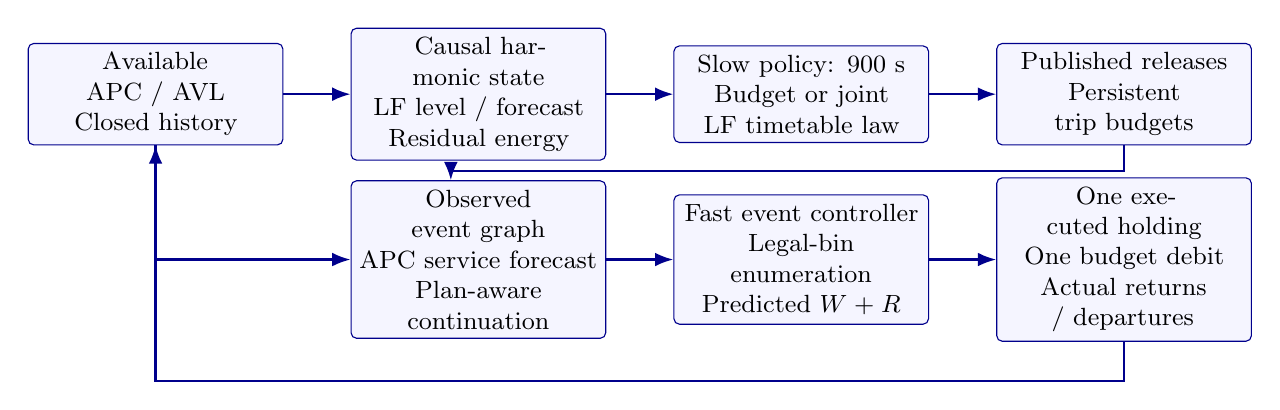
\begin{tikzpicture}[font=\small,>=Latex,
 box/.style={draw=blue!55!black,rounded corners=2pt,fill=blue!4,align=center,minimum height=1.0cm,text width=3.0cm},
 arr/.style={->,thick,blue!55!black}]
\node[box] (data) at (0,0) {Available APC / AVL\\Closed history};
\node[box] (freq) at (4.1,0) {Causal harmonic state\\LF level / forecast\\Residual energy};
\node[box] (slow) at (8.2,0) {Slow policy: 900 s\\Budget or joint\\LF timetable law};
\node[box] (ledger) at (12.3,0) {Published releases\\Persistent trip budgets};
\node[box] (graph) at (4.1,-2.1) {Observed event graph\\APC service forecast\\Plan-aware continuation};
\node[box] (fast) at (8.2,-2.1) {Fast event controller\\Legal-bin enumeration\\Predicted $W+R$};
\node[box] (physical) at (12.3,-2.1) {One executed holding\\One budget debit\\Actual returns / departures};
\draw[arr] (data)--(freq);
\draw[arr] (freq)--(slow);
\draw[arr] (slow)--(ledger);
\draw[arr] (data.south) |- (graph.west);
\draw[arr] (ledger.south) -- ++(0,-.32) -| ([xshift=-.35cm]graph.north);
\draw[arr] (graph)--(fast);
\draw[arr] (fast)--(physical);
\draw[arr] (physical.south) -- ++(0,-.5) -| (data.south);
\end{tikzpicture}
\caption{Shared information and resource interface, reused from the development architecture. Manual joint fixes the slow mode to joint; the learned comparator selects budget or joint. The fast controller uses APC/AVL, published plans, and remaining budgets. Frequency summaries enter the slow state and timetable law. Physical events update observations and resource accounting.}
\label{fig:architecture}
\end{figure*}

\subsection{Causal Frequency Summaries}
The frequency tracker forms closed-bin APC signals and maintains a causal harmonic state. For a nonnegative observed rate $x_n$, let $z_n=\log(1+x_n)$ and let $\phi_n$ contain an intercept, a temporal trend, and harmonic basis terms. A recursive least-squares update has the form
\begin{align}
 k_n&=\frac{P_{n-1}\phi_n}{\rho+\phi_n^\top P_{n-1}\phi_n},\\
 \theta_n&=\theta_{n-1}+k_n(z_n-\phi_n^\top\theta_{n-1}),\\
 P_n&=\rho^{-1}(P_{n-1}-k_n\phi_n^\top P_{n-1}).
\end{align}
Here $\rho$ is the recursive estimator's forgetting factor, distinct from budget retention $\rho_B$. The transformed fitted value supplies a nonnegative low-frequency (LF) summary $L_n$. A residual is formed against the \emph{pre-update} prediction, and its smoothed value and high-frequency (HF) energy are retained. Thus the fitted low component and smoothed residual are not an exact additive reconstruction of the raw count. A future LF summary is obtained by evaluating the fitted state at the future harmonic phase, without incorporating future observations.

The implemented slow state includes global low demand, its slope, a low-frequency forecast, and high-frequency energy. The timetable rule uses the global low level and forecast. Station-specific short-window arrival-rate estimates in the fast graph are obtained separately from APC clearance intervals. They have units of passengers per second and are not interchangeable with boarding-bin residuals. This separation avoids adding quantities with different sampling and exposure meanings.

\subsection{Bounded Dynamic Timetable Revision}
The slow manager begins at 7200 s and considers publication every 900 s. For each direction, a revision concerns the next mutable departure and preserves the following departure as an anchor. Write $p_1$ for the next public release, $p_2$ for the following public release, and $d_-$ for the preceding actual departure. Let $L_t$ and $F_t$ be the currently supported low-frequency level and forecast. Define
\begin{align}
 \omega_t&=\clip((p_2-t)/1800,0,1),\\
 \ell_t&=\pos{L_t},\qquad r_t=\pos{(1-\omega_t)L_t+\omega_t F_t},\\
 \tau^*&=\frac{\ell_t d_-+r_t p_2}{\ell_t+r_t}.
 \label{eq:timetable}
\end{align}
If the frequency estimate is unsupported, equal weights replace $\ell_t$ and $r_t$. The proposed release is restricted to a $\pm30$ s shift around $p_1$, then constrained by the current time, a 180 s minimum separation from the preceding published release, and a 180 s separation from the anchor. The executable value is rounded upward to the simulator's integer-second clock. Both the revised trip's target headway and the anchor's following target headway are updated.

A revision requires two mutable future departures within the publication window, sufficient completed-trip history, and a compatible vehicle-supply estimate. A trip that has already become operationally committed is not rewritten. The rule evaluates supply from available vehicles and forecast returning vehicles; it does not create an additional vehicle or reserve an unobserved return. Manual joint always enables this law and the budget mechanism. The optional learned supervisor controls permission to invoke the law rather than directly optimizing timetable entries.

\subsection{Persistent Holding Budgets}
For each active vehicle--trip pair $i$, the manager estimates the normal remaining command exposure $C_i$ from the number of remaining controls and the median command seconds per control in at least three completed eligible trips of the same direction. A return estimate separates the remaining non-holding running and service component, irrevocable commands, and the physical overhead of control events. It is matched to an upcoming trip within a 2700 s supply look-ahead.

Let $\widehat r_i^{\mathrm{ord}}$ be the estimated ordinary return time, and $p_{j(i)}$ the public departure of the matched trip. The estimated supply pressure and proposed remaining allowance are
\begin{align}
 P_i&=\pos{\widehat r_i^{\mathrm{ord}}+1-p_{j(i)}},\\
 \widetilde B_i&=\left\lceil\max(\rho_B C_i,C_i-P_i)\right\rceil.
 \label{eq:budget}
\end{align}
The default uses $\rho_B=0.5$; the independent configuration study also evaluates 0.25 without retraining. This retention floor preserves a fraction of the estimated ordinary command exposure; a larger value permits more holding time at the same supply pressure. The ordinary exposure is estimated from the policy's own completed-trip history, not an externally fixed regularity requirement. The allowance is vehicle time, not a vehicle or driver fraction. Only active trips with positive pressure, positive normal exposure, and remaining control opportunities receive a new allowance. If one already exists, publication takes $\min(B_i,\widetilde B_i)$ rather than replenishing it. At final submission of a command,
\begin{equation}
 B_i\leftarrow B_i-h_e,\qquad h_e\leq B_i^{\mathrm{before}}.
 \label{eq:debit}
\end{equation}
The allowance is closed when that trip returns. It persists across changes in the upper mode and across all remaining control points.

Budget accounting uses command seconds. In the simulator, a zero command still occupies one physical tick at a control point. Thus physical residence is $\max(1,h_e)$ for a submitted command, with corresponding automatic zero ticks at unrequested controls. Treating residence as identical to the budget debit would change the executed model. The return predictor estimates this overhead separately; it does not claim that subtracting one budget second always advances a return by one second.

\subsection{Fast Holding with a Common Continuation}
The native bilateral request uses forward departure spacing $g_f$ and a causal estimate of following-bus action-ready spacing $g_b$. When both are supported, its continuous request is $0.25(g_b-g_f)/2$. Without following-bus evidence it uses $0.25(T-g_f)$ for the trip target $T$; without forward evidence it requests zero. The result is clipped to $[0,45]$ s and mapped to the nearest original legal bin, with ties selecting the shorter command. Follower identity and timing use current telemetry and completed observations, not future return labels.

At a controllable event, the fast layer constructs a graph from the same current observations, published plans, and budget ledger. Its reference is the native bilateral rule projected onto the remaining allowance. If the native command is $h_e^{\mathrm{nat}}$, the projection is
\begin{equation}
 \bar h_e=\max\{h\in\mathcal H_e:h\leq h_e^{\mathrm{nat}},\ h\leq B_i\},
 \label{eq:projection}
\end{equation}
where the budget restriction is omitted for an unbudgeted trip. The rule's original legal mask is preserved. The current controller enumerates the legal members of $\{0,5,10,15,20,30,45\}$ s, using the same future native continuation and a separate copy of the ledger for each evaluation. The selected action minimizes predicted $W+R$ over candidates that satisfy the frozen relative feasibility conditions: predicted CV$^2$, relevant vehicle return times, subsequent departure times, and trip departure delays must not exceed their reference values. Coverage must be complete for the required events. The first executable command is applied; future actions remain predictions.

Published releases affect terminal events and downstream supply matching in the graph. Budget depletion changes later available commands. These dependencies mean that the two layers interact through a shared feasible set, even if the immediate passenger-cost ordering of the current holding candidates does not change. Every trial starts from the same remaining allowance, so searching more candidates does not spend physical budget. Only the executed command debits the live ledger.

If the predictive reference lacks the required support, the controller uses the budget-feasible native command. This fallback is an operational part of the method. An enumeration can be exact over the current finite library and still fail to identify the best real-world action, because the future continuation and demand estimates are approximate. We therefore distinguish search completeness from prediction accuracy and from actual transport benefit.

\subsection{Optional Learned Publication-Permission Comparator}
The upper action set is $\mathcal A=\{\mathrm{budget},\mathrm{joint}\}$. Both modes permit persistent budgets; only the joint mode permits a new timetable revision. The 180-dimensional state contains the time, fleet load, frequency summaries, accumulated arrival-headway moments, public-delay debt, the previous mode, directional supply and plan summaries, completed-trip history, and telemetry and remaining allowances for the 12 vehicles. Fixed divisors normalize these fields. The same canonical action labels are used in the actor, critic, replay, previous-action encoding, and execution.

The reward is the negative increment of~\eqref{eq:objective} over a slow interval, with $\gamma=1$ and the final interval closed after the service tail. A discrete maximum-entropy actor--critic uses twin critics, a 64-unit hidden width and fixed entropy temperature $10^{-5}$. Evaluation is deterministic. The complete optimization settings and update equations are provided in the Supporting Information; this optimizer is a matched comparator, not the proposed contribution.

\begin{algorithm}[t]
\caption{The shared timetable--holding interface}
\label{alg:control}
\begin{algorithmic}[1]
\STATE Update histories from newly available APC/AVL events.
\IF{a new slow publication time has been reached}
\STATE Use joint for manual control, or select budget/joint with the frozen supervisor.
\STATE Issue or tighten trip budgets using~\eqref{eq:budget}.
\IF{joint is selected and a plan revision is supported}
\STATE Publish the bounded release and its two target headways.
\ENDIF
\ENDIF
\IF{a vehicle requests a holding action}
\STATE Build the observed graph with current plans and budgets.
\STATE Project the native reference using~\eqref{eq:projection}.
\STATE Enumerate current legal candidates with separate ledgers.
\STATE Select the lowest-cost feasible action or reference fallback.
\STATE Submit one command and debit its live trip allowance once.
\ENDIF
\STATE Close the allowance when its physical trip returns.
\end{algorithmic}
\end{algorithm}

\subsection{Joint Credit Admission as a Development Candidate}
Pressure credit in~\eqref{eq:budget} restricts the continuation before the fast model checks relative feasibility. We therefore evaluate a separate candidate that treats new credit itself as a decision. At the slow clock, the original formula proposes an allowance without imposing it. At the proposing cycle's next supported holding query, the unchanged fast selector with existing credit produces a common no-new-tightening reference. We enumerate current legal commands under the proposed credit and require their continuations to meet the same reference's passenger-cost, CV$^2$, return, next-launch, and dispatch-delay conditions. The lowest predicted passenger cost is preferred; exact cost ties prefer lower total public delay. Only a strict cost or delay improvement admits the new allowance.

Commands submitted between proposal and admission debit the proposed remainder. A request expires at the next publication or physical return. Unsupported evidence imposes no new tightening; existing credit and irreversible commands remain unchanged. The chosen allowance is committed before its current command is submitted. This candidate changes credit admission, not the demand predictor, legal bins, cost weights, or fleet.

\subsection{Operational Coupling}
The architecture makes two interactions explicit: slow releases alter fast resource feasibility, and fast holding consumes vehicle time that constrains later releases. It also exposes a useful distinction between \emph{permission} and \emph{dose}. Selecting joint does not guarantee that a plan will be revised; the law may reject a publication, produce the same integer-second release, or be unable to influence an already committed trip. An upper action count is therefore insufficient evidence of timetable control. We record published revisions, binding to actual departures, and changes relative to matched control paths.

The implemented frequency pathway runs from the causal summary to the slow state or timetable law, and then from published plans and budgets to fast control. The architecture in Fig.~\ref{fig:architecture} depicts these paths. The representation and supervisor comparisons evaluate their incremental effects separately from the budget-setting contrast.

\section{Accounting and Comparison Semantics}
\label{sec:properties}
If a trip receives allowance $B_0$, legal command debits $h_e$ and later
nonnegative tightenings $u_v$ satisfy
\begin{equation}
 B_{\rm rem}=B_0-\sum_eh_e-\sum_vu_v\geq0.
 \label{eq:budget_identity}
\end{equation}
This is an accounting invariant, not a vehicle return-time or passenger-cost
guarantee. The same ordered debit rule operates in each trial continuation and
in physical execution. An anchored timetable revision redistributes two
adjacent targets without adding a trip or vehicle. Full derivations are in the
Supporting Information.

For the actual nonterminal arrival-headway prefix, let $n$, $S$ and $Q$ denote
the count, sum and squared sum. The shared population-moment statistic is
\begin{equation}
 \mathrm{CV}^2=\frac{nQ}{S^2}-1,\qquad n>0,\ S>0.
 \label{eq:cv_moments}
\end{equation}
The fast model adds a predicted suffix without counting an observed arrival
twice; terminal returns affect supply but not this statistic.

A relative feasibility guard protects its reference, not the decision that
created that reference. In the original method the reference already includes
published credit. The common-reference candidate asks the different question
of whether issuing new credit and taking its current action improve upon a
no-new-tightening continuation. Neither local comparison guarantees complete-day
non-harm under later closed-loop decisions. These distinct questions motivate
the separate allocation and admission experiments.

\section{Experimental Design}
\label{sec:experiments}
\subsection{Physical Contract and Endpoints}
All studies retained 12 physical vehicles and 262 scheduled trips, with 131 departures per direction at a public 360-s interval. The two directional schedules began 180 s apart. The simulator advanced in 1-s steps; the original seven holding bins were retained throughout. Demand was generated from the frozen hourly origin--destination template with stochastic demand perturbations. A demand-day identifier denotes a simulated realization, not an observed calendar service day.

Demand generation ended at 46,980 s. The evaluation contract allowed a 14,400-s service tail and a maximum horizon of 61,380 s, with earlier physical termination when service cleared. For $N$ passengers generated on the common demand realization, waiting and onboard exposure were $W/N$ and $R/N$, using the frozen one-second occupancy integrals. We call their sum \emph{restricted journey exposure}. It includes accounted waiting by generated passengers who remain unserved, rather than conditioning on completed journeys. Individual timestamp-derived durations used for tail percentiles are kept separate from these grid-integrated means; neither definition is silently substituted for the other.

For public release $p_j$, actual departure $d_j$, and the observed time $e_j$ when the trip first became dispatch-eligible under its operational plan, the reported operational measures were
\begin{align}
 D_{\rm pub}&=\sum_{j\in\mathcal T}\max(0,d_j-p_j),\\
 \overline D_{\rm ready}&=\frac{1}{262}\sum_{j\in\mathcal T}(d_j-e_j).
\end{align}
Public delay is a daily total; readiness delay is seconds per scheduled trip. The public references were immutable, so changing an operational release could not redefine away measured lateness. Positive public delay does not penalize an early departure symmetrically. Actual nonterminal arrival CV$^2$ used~\eqref{eq:cv_moments}. Commanded and executed holding, trip completion, and physical returns were also checked.

\subsection{Separate Studies and Statistical Units}
\begin{table}[t]
\centering\footnotesize
\caption{Evaluation panels. Calibration, engineering paths and learning collections are accounted for separately.}
\label{tab:panels}
\begin{tabularx}{\columnwidth}{@{}lYrr@{}}
\toprule
Study & Question & Days & Paths\\
\midrule
A & Independent budget and representation tests & 16 & 80\\
B & Explicit-retention learner development & 4 & 24\\
C & Independent simple-limit comparison & 16 & 80\\
D & Joint-credit admission development & 4 & 24\\
E & Factorial and demand-condition supplement & 16 & 144\\
\bottomrule
\end{tabularx}
\end{table}

Study~A evaluated the preselected K4 supervisor and the same-seed matched K0 supervisor at their final training checkpoints. Each original learner had 32 training demand days in eight four-day batches with 192 updates per batch. The selected seed was 314011; no new seed or checkpoint was selected on the 16 test days. The five arms were K4 and manual joint at each of $\rho_B=.50$ and $.25$, and K0 at $.50$. K0 retained trend, online adaptation and innovation statistics. Removing harmonics also reduced estimator capacity, so this was a defined representation ablation rather than removal of every temporal feature.

Study~B trained two new learners with identical 181-channel architectures, initialization, day/retention assignments and update budgets. Each used 32 original training days and 1,536 updates. The final channel was the day's retention for the explicit learner and zero for the implicit learner; both still observed physical remaining credit. Each learner was evaluated at both retentions on four new development days, with manual joint as a control. This tested an explicit budget-context change without changing the two publication modes.

Study~C froze manual joint and the fast model, then compared pressure credit at $.50$ with static remaining-trip credit and a per-stop cap. A static setting issued $\lceil c n_i\rceil$ seconds once, where $n_i$ was the number of uncommitted controls at first supported publication. A stop cap limited each subsequent legal command on an admitted cycle. Both restrictions also entered plan-supply forecasts and model continuation. All policies used the same publication start and completed-history requirements; their allocation rules could admit different cycles.

Only four previously consumed development days calibrated the simple controls. Static settings were $c\in\{0,2.5,5,7.5,10,15,20,30,45\}$ s per remaining control, and caps were $\{0,5,10,15,20,30,45\}$ s. All 64 calibration paths were retained. For each family, the closest realized-holding brackets around the pressure mean were chosen; an ex-ante daily mixture matched that development mean. The frozen static mixture used 7.5 and 10 with probabilities .466709 and .533291, and the cap mixture used 10 and 15 with probabilities .210341 and .789659. The expected daily endpoint was obtained by evaluating both whole-day components and applying these fixed probabilities. It was not formed by mixing actions along one trajectory. No test-day reweighting occurred.

Study~D froze the joint-admission candidate and reused those original mixture probabilities. Four further development days evaluated six physical arms: the candidate, pressure credit, both static settings, and both caps. Engineering first checked exact pressure reproduction and the new selector's no-proposal behavior, then verified a real candidate path and its chronological credit ledger. Performance on that old engineering day did not tune the candidate or gate its development screen.

Study~E adds a frozen factorial and operating-condition supplement without selecting another controller. Four conditions retain nominal demand, multiply demand by .8 or 1.2, or shift the hourly demand lookup by one hour. Each uses four distinct, previously unconsumed demand days. The nine physical arms are the four model-controller corners (fixed timetable/no credit, timetable only, credit only, and joint), the four already frozen simple-limit components, and fixed360 with the native bilateral holding rule. The four corners share the same fast model, costs, seven legal actions and retention .50. The bilateral arm executes its original rule with no model overrides. Comparing joint against credit-only isolates timetable revision given credit; joint against timetable-only isolates credit given revision; the difference-in-differences measures their interaction. These conditional effects are not claims about a learned supervisor.

Study~E uses the original mixture probabilities without new intensity matching.
All four simple components are reported, rather than selecting a favorable one
after evaluation. Paired intervals use 10,000 day-bootstrap draws with seed
4041110 and are descriptive within each four-day condition. The native
generator uses demand-noise parameter .15 and samples from the peak-offset list
$(-1,0,0,0,+1)$ h. Nominal, light and heavy retain this offset draw; rushshift
fixes it to $+1$ h. The latter reweights an existing pattern rather than
introducing an unseen peak shape. Route speeds use native noise parameter 1.5
and a day-seeded scenario tape at fixed exogenous update times, shared within
each day's policy comparison. The perturbation law is unchanged: running-noise
intensity, route geometry and fleet size are not additional factors.

The 144 distinct formal paths in Study~E include one native baseline used for the runtime engineering check; two further old-day starts are charged separately, including one failed observation capture. The total allowance is 146 traffic starts, with no automatic retry. Frozen pressure control exactly reproduced its old archived path before the independent runtime was released.

\subsection{Pairing, Hypotheses and Accounting}
The timetable component changes the mutable release and its two adjacent target headways. Its factorial effect therefore includes both terminal timing and the subsequent response to those targets. It is not an isolated mediation estimate for a changed actual departure.

Policies within a day shared the demand realization, public clocks and 5,200 common sampler events. Actual action submission, execution, returns and the fixed trip roster were checked before statistical aggregation. The independent studies sampled demand days, not independent continuation futures or fresh learning seeds. Day means received equal weight.

Study~A retained its two prespecified primary propositions. The budget-service proposition required the learned $.25-.50$ journey upper bound to be below zero and its readiness upper bound to be non-positive; actual CV$^2$ was reported as the operating tradeoff. The harmonic proposition required the K4$-$K0 journey upper bound to be below zero. Archived intervals used 10,000 paired day-bootstrap draws and seed 4000201. Their 95\% two-sided upper endpoints supplied the frozen 97.5\% one-sided bounds. Supervisor and additional endpoint comparisons were reported separately.

Study~C asked a stricter question: pressure credit had to reduce public dispatch delay while preserving actual CV$^2$ against each simple family. Its zero-margin protections and 97.5\% one-sided bounds were frozen before testing, with multiplicity handled across the two families. It used 10,000 paired demand-day bootstrap draws and seed 40211010. Passing required both joint comparisons, rather than selecting the more favorable one.

Study~D was a development screen, not a repeat confirmation. Its fixed criterion required lower mean public delay and non-higher mean CV$^2$ against both simple mixtures. Four-day bootstrap intervals were descriptive, with 10,000 archived draws and seed 40311010. The candidate's comparison with old pressure and its passenger costs were retained without requiring dominance of every operating point. A failed screen did not authorize a new retention, forecast repair or confirmation expansion.

All tables below format server-computed archived estimates directly. They do not pool days across studies or replace an original gate with a supplemental interval. Study~E's four conditions are reported separately, not counted as 16 replications of one nominal setting.

\section{Results}
\subsection{Budget Retention Reproduced an Operating Tradeoff}
\begin{table*}[t]
\centering
\footnotesize
\caption{Independent budget study: tighter retention ($.25-.50$), 16 paired demand days. Estimates and archived 95\% day-bootstrap intervals. Negative means lower.}
\label{tab:budget}
\setlength{\tabcolsep}{4pt}
\begin{tabularx}{\textwidth}{@{}lYYYY@{}}
\toprule
Comparison & Journey (s/person) & Readiness (s/trip) & Public delay (s/day) & Actual CV$^2$ \\
\midrule
Learned supervisor & \shortstack[r]{$-1.645$\\{\scriptsize $[-3.074,-0.070]$}} & \shortstack[r]{$-3.804$\\{\scriptsize $[-4.781,-2.915]$}} & \shortstack[r]{$-1001.62$\\{\scriptsize $[-1255.06,-771.75]$}} & \shortstack[r]{$+0.005646$\\{\scriptsize $[+0.003261,+0.009176]$}} \\[3pt]
Manual joint & \shortstack[r]{$-2.396$\\{\scriptsize $[-3.771,-0.976]$}} & \shortstack[r]{$-4.540$\\{\scriptsize $[-5.579,-3.595]$}} & \shortstack[r]{$-1185.44$\\{\scriptsize $[-1457.63,-939.62]$}} & \shortstack[r]{$+0.003025$\\{\scriptsize $[+0.001410,+0.004741]$}} \\[3pt]
\bottomrule
\end{tabularx}
\end{table*}

On the 16 independent days in Study~A, reducing retention from .50 to .25 lowered journey exposure and readiness delay under both learned and manual supervision (Table~\ref{tab:budget}). The learned controller's journey difference was $-1.645$ s/passenger, with interval $[-3.074,-0.070]$; the manual contrast was $-2.396$ s/passenger, with interval $[-3.771,-0.976]$. The corresponding actual CV$^2$ differences were positive for both controllers. The original budget-service proposition passed with its registered interpretation: improved passenger exposure and circulation accompanied by worse regularity.

These within-controller contrasts establish a configuration effect, not a learned-policy increment. In particular, manual joint also benefited from tighter retention. The public-delay and readiness columns describe related parts of the same vehicle-supply chain and are not independent replications of an operating benefit.

\begin{figure*}[t]
\centering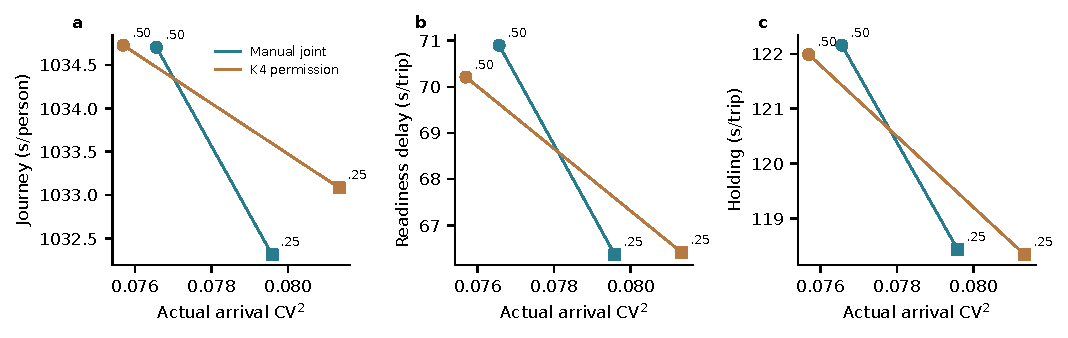
\includegraphics[width=\textwidth]{figures/budget_retention.pdf}
\caption{Budget retention and the service--circulation tradeoff on the same 16 independent demand days. Circles and squares denote retention .50 and .25, respectively. Each point is a complete-day mean; line segments connect only the two frozen settings and are not an optimized frontier. Reduced holding accompanies lower journey exposure and readiness delay but higher actual CV$^2$. Paired differences and uncertainty are reported in Table~\ref{tab:budget}.}
\label{fig:retention}
\end{figure*}

\subsection{Learning and Harmonic Inputs Had Different Evidence Boundaries}
\begin{table*}[t]
\centering
\footnotesize
\caption{Independent representation and supervisor comparisons, 16 paired demand days. K4 retains harmonics; K0 retains trend, online adaptation and innovation statistics. Intervals crossing zero are not equivalence tests.}
\label{tab:supervisor}
\setlength{\tabcolsep}{4pt}
\begin{tabularx}{\textwidth}{@{}lYYY@{}}
\toprule
Comparison & Journey (s/person) & Readiness (s/trip) & Actual CV$^2$ \\
\midrule
K4$-$manual, $\rho_B=.50$ & \shortstack[r]{$+0.022$\\{\scriptsize $[-0.608,+0.584]$}} & \shortstack[r]{$-0.690$\\{\scriptsize $[-1.400,-0.048]$}} & \shortstack[r]{$-0.000867$\\{\scriptsize $[-0.002202,+0.000353]$}} \\[3pt]
K4$-$manual, $\rho_B=.25$ & \shortstack[r]{$+0.773$\\{\scriptsize $[+0.075,+1.458]$}} & \shortstack[r]{$+0.045$\\{\scriptsize $[-0.620,+0.570]$}} & \shortstack[r]{$+0.001754$\\{\scriptsize $[-0.000713,+0.005083]$}} \\[3pt]
K4$-$K0, $\rho_B=.50$ & \shortstack[r]{$-0.562$\\{\scriptsize $[-1.567,+0.352]$}} & \shortstack[r]{$-0.104$\\{\scriptsize $[-0.597,+0.436]$}} & \shortstack[r]{$-0.000937$\\{\scriptsize $[-0.001668,-0.000175]$}} \\[3pt]
\bottomrule
\end{tabularx}
\end{table*}

At matched default retention, K4$-$manual journey exposure was $+0.022$ s/passenger with interval $[-0.608,0.584]$ (Table~\ref{tab:supervisor}). At $.25$, the difference was $+0.773$ s/passenger with interval $[0.075,1.458]$. Thus the independent panel did not establish a learned-supervisor journey advantage; the tighter setting favored the manual comparator on that endpoint. An interval spanning zero at the default setting did not establish equivalence.

The independent K4$-$K0 journey estimate was $-0.562$ s/passenger with interval $[-1.567,0.352]$, so the primary harmonic-journey proposition failed. The secondary actual-CV$^2$ interval favored K4 (Table~\ref{tab:supervisor}). These endpoints retain their separate status: the secondary regularity result does not replace the failed journey criterion.

Study~B produced the same executed policy as manual joint. Both newly trained learners selected joint at every one of their 47 publications in each of the 16 learned development paths. Their waiting, onboard, journey, readiness, public delay and CV$^2$ differences from manual joint were exactly zero at the matching retention on all four days. Each learner received 1,536 updates. The explicit-retention development screen therefore failed. Joint selection still invoked a demand- and vehicle-dependent timetable law; it did not imply a fixed timetable or an inactive controller.

\subsection{Pressure Credit Improved Delay but Failed Regularity Protection}
\begin{table*}[t]
\centering
\footnotesize
\caption{Pressure credit minus frozen simple-limit mixtures on 16 new paired demand days. Weights matched development holding exposure, not test-day holding or regularity. Both delay tests pass and both CV$^2$ protections fail.}
\label{tab:limits}
\setlength{\tabcolsep}{4pt}
\begin{tabularx}{\textwidth}{@{}lYYYY@{}}
\toprule
Comparison & Public delay (s/day) & Actual CV$^2$ & Journey (s/person) & Readiness (s/trip) \\
\midrule
Static trip credit & \shortstack[r]{$-3744.15$\\{\scriptsize $[-4401.41,-3025.06]$}} & \shortstack[r]{$+0.006573$\\{\scriptsize $[+0.004168,+0.008979]$}} & \shortstack[r]{$-4.761$\\{\scriptsize $[-6.670,-2.884]$}} & \shortstack[r]{$-14.354$\\{\scriptsize $[-16.858,-11.610]$}} \\[3pt]
Per-stop cap & \shortstack[r]{$-3123.80$\\{\scriptsize $[-3791.96,-2377.11]$}} & \shortstack[r]{$+0.006883$\\{\scriptsize $[+0.004661,+0.009121]$}} & \shortstack[r]{$-0.056$\\{\scriptsize $[-1.835,+1.849]$}} & \shortstack[r]{$-11.975$\\{\scriptsize $[-14.511,-9.145]$}} \\[3pt]
\bottomrule
\end{tabularx}
\end{table*}

On Study~C's 16 new days, pressure credit reduced public delay relative to both simple mixtures (Table~\ref{tab:limits}). The differences were $-3744.15$ s/day against static credit and $-3123.80$ s/day against the stop cap. Both delay bounds were below zero, but both actual-CV$^2$ intervals were above zero. Each joint gate failed under its original criterion.

The journey contrast against static credit was $-4.761$ s/passenger with interval $[-6.670,-2.884]$. Against the stop cap it was $-0.056$, with interval $[-1.835,1.849]$. Waiting intervals spanned zero for both families. Thus a passenger advantage was supported against one defined simple mixture, not uniformly against both.

Development exposure matching did not ensure matched test exposure. Pressure credit used 3.259 fewer holding seconds per trip than the static mixture and 1.797 fewer than the cap mixture on the new days. It improved delay on 16/16 and 15/16 days, respectively, while worsening CV$^2$ on 14/16 and 15/16 days. The failed protection was therefore directional across the panel, rather than driven by one adverse day.

\begin{figure*}[t]
\centering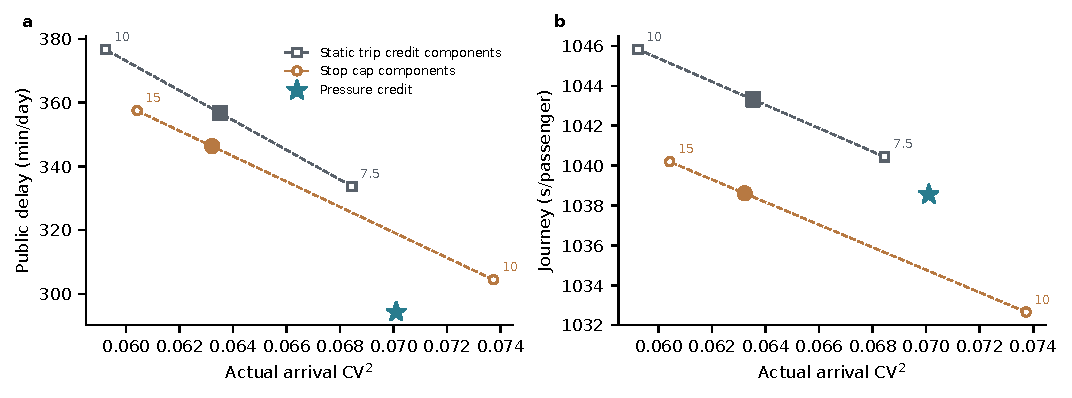
\includegraphics[width=\textwidth]{figures/independent_tradeoff.pdf}
\caption{Operating points on the original 16 independent days. Hollow points show the four frozen simple-limit components; filled points show their original ex-ante daily mixtures. Dashed segments span expectations of whole-day randomization, not mixing actions within a trip. Pressure credit lowers dispatch delay against both mixtures but increases CV$^2$. Component comparisons reveal a different delay--regularity geometry from the journey--regularity geometry. Paired mixture uncertainty is in Table~\ref{tab:limits}; these points are not a certified optimal frontier and no new mixture is selected.}
\label{fig:independent_tradeoff}
\end{figure*}

The finite calibration grid (Supporting Fig.~S1) and the independent operating points (Fig.~\ref{fig:independent_tradeoff}) answer different questions. The grid contains promising pressure-credit configurations on consumed development days, but does not certify a frontier on unseen days. The unchanged independent mixtures expose the resulting regularity cost without test-day intensity matching.

Reporting the four component policies also reveals why actual holding alone does not order the outcomes. Against the 10-s stop cap, pressure used 14.210 more holding seconds per trip while reducing public delay by 608.94 s/day and actual CV$^2$ by 0.003636; journey exposure increased by 5.900 s/passenger. Against the 7.5-s static setting, pressure also used more holding, but lowered journey and delay while the CV$^2$ interval crossed zero. Against the two looser components, pressure reduced holding and delay but worsened CV$^2$. These secondary contrasts are reported together in the Supporting Information. They distinguish operating dimensions without selecting a new mixture or overturning the original joint failures.

\subsection{Joint Credit and Operating Cost}
\begin{table*}[t]
\centering
\footnotesize
\caption{Common-reference joint-credit candidate minus each comparator on four NEW development days. Intervals are descriptive. This is not independent confirmation. Both simple-control delay screens fail; both mean CV$^2$ protections pass.}
\label{tab:joint}
\setlength{\tabcolsep}{4pt}
\begin{tabularx}{\textwidth}{@{}lYYYY@{}}
\toprule
Comparison & Public delay (s/day) & Actual CV$^2$ & Journey (s/person) & Holding (s/trip) \\
\midrule
Static mixture & \shortstack[r]{$+5917.10$\\{\scriptsize $[+3715.79,+8773.66]$}} & \shortstack[r]{$-0.013690$\\{\scriptsize $[-0.016188,-0.009969]$}} & \shortstack[r]{$+6.803$\\{\scriptsize $[+0.889,+15.613]$}} & \shortstack[r]{$+22.333$\\{\scriptsize $[+18.603,+26.062]$}} \\[3pt]
Stop-cap mixture & \shortstack[r]{$+6165.45$\\{\scriptsize $[+4157.09,+8765.84]$}} & \shortstack[r]{$-0.012680$\\{\scriptsize $[-0.016640,-0.008721]$}} & \shortstack[r]{$+10.744$\\{\scriptsize $[+4.138,+20.729]$}} & \shortstack[r]{$+24.454$\\{\scriptsize $[+21.333,+27.574]$}} \\[3pt]
Old pressure & \shortstack[r]{$+9918.50$\\{\scriptsize $[+6623.00,+13315.00]$}} & \shortstack[r]{$-0.020795$\\{\scriptsize $[-0.032846,-0.012465]$}} & \shortstack[r]{$+12.768$\\{\scriptsize $[+1.377,+25.861]$}} & \shortstack[r]{$+26.250$\\{\scriptsize $[+19.585,+32.352]$}} \\[3pt]
\bottomrule
\end{tabularx}
\end{table*}

The Study~D candidate improved actual CV$^2$ against both simple mixtures on all four new development days (Table~\ref{tab:joint}). However, journey exposure and public delay were worse on every day against each mixture. The mean-delay conditions failed and both mean-CV$^2$ protections passed; the overall development screen failed.

The execution record showed 985 evaluated credit requests: 34 were admitted, 919 offered no joint improvement under the common reference, and 32 had an unsupported reference. All admitted budgets passed chronological accounting. Actual holding averaged 146.594 s/trip, compared with 120.344 for old pressure. Relative to old pressure, the candidate's CV$^2$ decreased by 0.020795, while journey exposure increased by 12.768 s/passenger and public delay increased by 9918.50 s/day. The candidate was closed without changing its constraints or opening independent confirmation.

\subsection{Operating Conditions Separate Budget and Timetable Effects}
\begin{table*}[t]
\centering\footnotesize
\caption{Conditional timetable and budget effects on four new paired demand days per regime. Timetable means joint minus budget-only; budget means joint minus timetable-only. Day-bootstrap intervals are descriptive, not a replacement for the original confirmation gates.}
\label{tab:factorial}
\setlength{\tabcolsep}{4pt}
\begin{tabularx}{\textwidth}{@{}llYYYY@{}}\toprule
Regime & Added component & Journey (s/person) & Public delay (min/day) & Readiness (s/trip) & Actual CV$^2$ \\ \midrule
nominal & Timetable given budget & \shortstack[r]{$+2.013$\\{\scriptsize $[+0.886,+3.847]$}} & \shortstack[r]{$+3.41$\\{\scriptsize $[+0.53,+6.29]$}} & \shortstack[r]{$+0.33$\\{\scriptsize $[-0.47,+1.12]$}} & \shortstack[r]{$+0.001951$\\{\scriptsize $[+0.000400,+0.003502]$}} \\[2pt]
nominal & Budget given timetable & \shortstack[r]{$-6.887$\\{\scriptsize $[-10.587,-0.817]$}} & \shortstack[r]{$-142.58$\\{\scriptsize $[-157.00,-128.17]$}} & \shortstack[r]{$-32.69$\\{\scriptsize $[-36.10,-29.28]$}} & \shortstack[r]{$+0.032276$\\{\scriptsize $[+0.026438,+0.037888]$}} \\[2pt]
light & Timetable given budget & \shortstack[r]{$+0.951$\\{\scriptsize $[-0.257,+2.408]$}} & \shortstack[r]{$+9.70$\\{\scriptsize $[+5.68,+14.62]$}} & \shortstack[r]{$+1.62$\\{\scriptsize $[+0.66,+2.83]$}} & \shortstack[r]{$+0.002047$\\{\scriptsize $[-0.000720,+0.005999]$}} \\[2pt]
light & Budget given timetable & \shortstack[r]{$-4.005$\\{\scriptsize $[-5.755,-1.853]$}} & \shortstack[r]{$-115.64$\\{\scriptsize $[-162.07,-73.84]$}} & \shortstack[r]{$-26.56$\\{\scriptsize $[-37.16,-17.05]$}} & \shortstack[r]{$+0.026161$\\{\scriptsize $[+0.011042,+0.050500]$}} \\[2pt]
heavy & Timetable given budget & \shortstack[r]{$-0.369$\\{\scriptsize $[-0.726,-0.069]$}} & \shortstack[r]{$+1.23$\\{\scriptsize $[+0.73,+1.95]$}} & \shortstack[r]{$-0.10$\\{\scriptsize $[-0.25,+0.07]$}} & \shortstack[r]{$+0.000629$\\{\scriptsize $[-0.000191,+0.001843]$}} \\[2pt]
heavy & Budget given timetable & \shortstack[r]{$-29.699$\\{\scriptsize $[-42.137,-20.531]$}} & \shortstack[r]{$-275.40$\\{\scriptsize $[-318.79,-231.33]$}} & \shortstack[r]{$-63.22$\\{\scriptsize $[-73.19,-53.07]$}} & \shortstack[r]{$+0.023173$\\{\scriptsize $[+0.018793,+0.028463]$}} \\[2pt]
rushshift & Timetable given budget & \shortstack[r]{$+1.217$\\{\scriptsize $[+0.037,+2.523]$}} & \shortstack[r]{$+5.25$\\{\scriptsize $[+0.78,+10.28]$}} & \shortstack[r]{$+0.76$\\{\scriptsize $[-0.23,+1.95]$}} & \shortstack[r]{$-0.000076$\\{\scriptsize $[-0.000725,+0.000574]$}} \\[2pt]
rushshift & Budget given timetable & \shortstack[r]{$-20.186$\\{\scriptsize $[-31.214,-12.149]$}} & \shortstack[r]{$-175.49$\\{\scriptsize $[-239.82,-138.47]$}} & \shortstack[r]{$-40.28$\\{\scriptsize $[-55.17,-31.70]$}} & \shortstack[r]{$+0.021655$\\{\scriptsize $[+0.016825,+0.025009]$}} \\[2pt]
\bottomrule\end{tabularx}
\end{table*}

Study~E completed all 144 paired paths. Relative to fixed360 with native bilateral holding, joint pressure control reduced journey exposure by 12.204, 6.841, 27.557 and 22.340 s/passenger under nominal, light, heavy and rush-shift demand, respectively (Fig.~\ref{fig:conditions}). Readiness delay fell by 37.57, 27.52, 60.26 and 43.58 s/trip. In all four regimes, however, actual CV$^2$ increased: the corresponding differences were 0.031353, 0.023641, 0.023758 and 0.020365. These are service--circulation gains accompanied by reduced regularity, not joint dominance.

\begin{figure*}[t]
\centering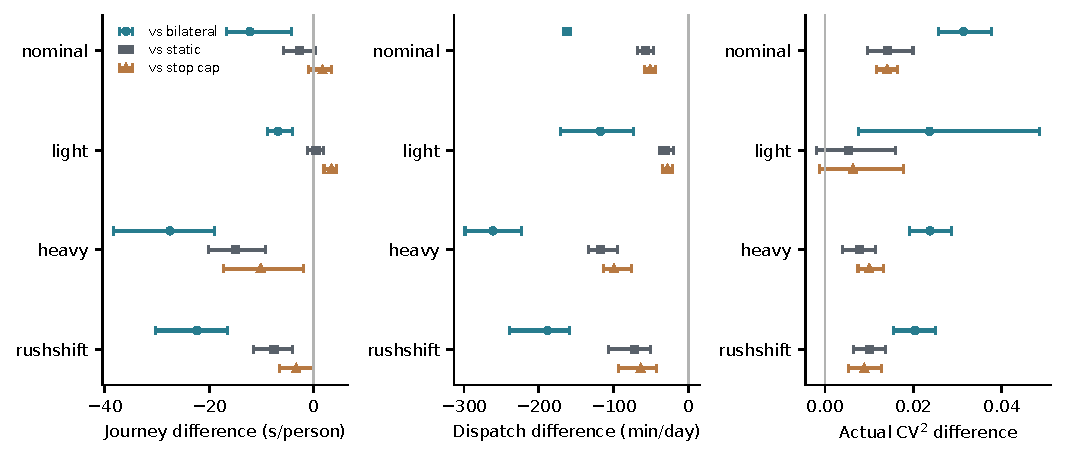
\includegraphics[width=\textwidth]{figures/regime_robustness.pdf}
\caption{Joint pressure control minus the native fixed360 bilateral baseline and the two frozen simple-limit mixtures under four operating conditions. Each estimate uses four independent paired demand days. Intervals are descriptive day bootstraps. No mixture or controller is selected from this panel. The CV$^2$ cost persists against native bilateral in every regime.}
\label{fig:conditions}
\end{figure*}

The model-controller factorial identifies pressure credit as the principal source of the circulation savings (Table~\ref{tab:factorial}). Adding the timetable law to budget-only control increased journey exposure by 2.013 s/passenger under nominal demand, 0.951 under light demand and 1.217 under rush shift; under heavy demand it reduced exposure by 0.369 s/passenger. The conditional timetable effect on public delay was adverse in all four regimes: $+204.5$, $+582.0$, $+74.0$ and $+314.75$ s/day. Active plan changes therefore did not establish a consistent incremental timetable benefit. All four corners and the interaction estimates are retained in the Supporting Information.

The original simple-mixture tradeoff also changed with operating conditions. Pressure lowered public delay relative to both mixtures in every regime. Journey exposure was worse than the stop-cap mixture in light demand by 3.423 s/passenger, with descriptive interval $[1.993,4.475]$, while heavy and rush-shift means favored pressure. Against the individual 10-s cap, the original panel's favorable delay--regularity combination did not recur uniformly: nominal CV$^2$ increased by 0.006184, whereas light CV$^2$ decreased by 0.008195 but journey exposure increased by 6.089 s/passenger. Reporting all components avoids interpreting one favorable projection as a general frontier improvement.

\subsection{Executed Supply Chains and Passenger Distribution}
The preregistered vehicle example was trip 31 of bus 9 on the first nominal day (Fig.~\ref{fig:chain}). Fixed-model and timetable-only control executed 105 s of holding, returned at 7616 s and launched the same vehicle on trip 42 at 7617 s. Budget-only and joint control executed 70 s, returned at 7585 s and launched at 7586 s. Thus a 35-s command reduction coincided with a 31-s earlier return and following departure; the timetable law added no change on this chain. The example demonstrates physical propagation under the frozen policies, rather than an isolated causal effect of holding with all subsequent states fixed.

\begin{figure*}[t]
\centering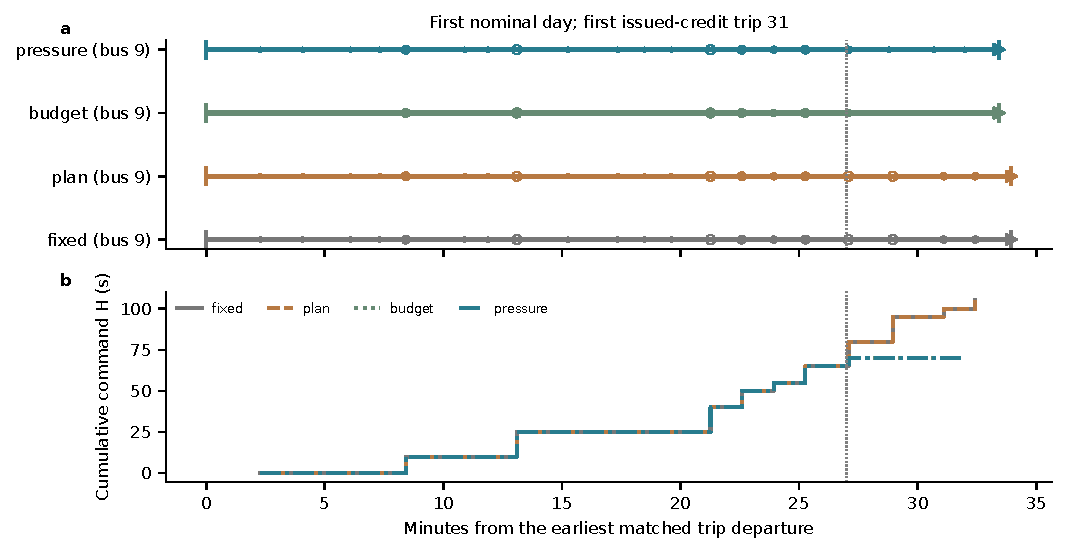
\includegraphics[width=.95\textwidth]{figures/vehicle_time_chain.pdf}
\caption{The predeclared first issued-credit trip on the first nominal day. Top: departure, physical return (right tick), and the assigned vehicle's next departure (triangle). Circles mark command submission times, with area increasing with holding. Bottom: cumulative commanded holding, all verified executed. The dotted line is the first credit publication. Fixed and plan-only coincide here, as do budget-only and joint. Future vehicle identities are evaluation labels, not controller inputs.}
\label{fig:chain}
\end{figure*}

Timetable revisions did reach execution elsewhere. On the four nominal days, joint had 19, 27, 26 and 20 revised final releases; 18, 26, 25 and 20 departures occurred exactly at those releases. Relative to budget-only, 75, 97, 72 and 57 actual departure times changed. This execution evidence excludes an inactive timetable as the explanation for its weak conditional result; it does not turn those changes into passenger gains. Trip/hour and same-vehicle-chain readouts are included with the source data.

Joint control reduced each day's journey P95 relative to native bilateral on average by 42.45, 17.92, 112.34 and 84.84 s across the four regimes. Mean gains did not benefit every cohort: on nominal days, several early origin stations had higher journey exposure despite the aggregate improvement (Supporting Information). Relative to the stop-cap mixture, light-demand journey P95 increased by 7.10 s, with descriptive interval $[2.91,11.28]$. These distributional results retain daily percentiles and passenger-weighted cohort means as distinct estimands.

Public-delay savings also coexisted with early departures. Joint averaged 7.00, 3.25, 9.75 and 5.00 early trips/day, with summed earliness of 15.75, 10.00, 33.25 and 10.50 s/day. Earliness is reported separately, not canceled against lateness. All vehicles completed their trips and no passengers remained onboard at the endpoint. Mean unserved counts were 0.50, 1.00, 744.75 and 47.00 passengers/day, respectively, with their fixed-horizon waiting retained; heavy-demand tail results therefore concern a capacity-stressed system rather than universal passenger completion.

\subsection{Engineering Validity and Computation}
All 80 Study~C test paths and all 24 Study~D development paths completed with the fixed fleet, full trip roster and valid physical accounting. The Study~D implementation also exactly reproduced the archived pressure path and its no-proposal selector path, with zero diagnostic roundoff in the registered comparison. One zero-traffic test-fixture failure was repaired and retained; it did not consume a traffic path. These checks support execution validity, separately from the scientific outcomes.

Archived full-day wall time in Study~C had median 21.26 min and maximum 29.35 min. In Study~D the corresponding values were 24.36 and 27.27 min, with 24 development paths running concurrently on Linux CPU nodes. These are batch experiment costs under the recorded server workloads, not per-query real-time latency guarantees.

Study~E used 146 charged starts: 144 successful formal paths and two old-day engineering attempts, including one preserved failed observation capture. The repaired engineering path exactly reproduced its archive. All formal paths ran from the standalone source snapshot. Their wall times had median 19.93 min, 95th percentile 26.87 min and maximum 28.78 min; native bilateral timings include passive graph observation. Across paths, the individual callback P95 ranged from 0.061 to 0.713 s. Queue and result-transfer time are excluded, and these observations do not guarantee one-second real-time execution.

Graph support averaged 85.70\%, 95.21\%, 0\% and 60.62\% under nominal, light, heavy and rush-shift demand. Under heavy demand, every query used native-rule fallback, still projected onto any remaining issued credit. Its 2,833 changes to native requests were budget projections rather than supported graph optima. The heavy-demand service gains cannot therefore be attributed to model-based action optimization. The primary exposure uses the frozen one-second occupancy integral; timestamp-based passenger readouts differed by about half a second per passenger, with paired offsets below $6\times10^{-12}$ s and no effect on the primary contrasts.

\section{Discussion}
\subsection{An Executable Interface Is Distinct from a Better Tradeoff}
The cumulative budget provides a common unit linking terminal supply forecasts, stop-level legal commands and physical execution. Its accounting identity answers whether the same limited resource was used throughout a trajectory. The independent retention study answers another question: how the operating point moved when that resource constraint changed. Both have positive evidence here. Neither by itself establishes that pressure-driven allocation outperforms a simpler restriction at the same service quality.

The independent simple-control comparison supplies that missing challenge. Pressure credit reduced dispatch delay but failed the registered regularity protections, while its journey benefit depended on the comparator. This is consistent with a useful operating configuration rather than a uniformly improved tradeoff. It also explains why holding exposure must be reported: matching average exposure on old days does not fix the exposure, service states or regularity of new trajectories.

The four-condition supplement strengthens the budget--circulation interpretation but narrows the coordination claim. Against native bilateral holding, journey and readiness improved in every condition while actual CV$^2$ worsened. The timetable law changed real departures, yet its conditional increment above budget-only control increased public delay in every condition. Conversely, the 10-s cap comparison changed geometry between nominal and light demand. There is no stable ordering in which the complex allocator is uniformly more effective, nor an empirical basis for claiming that timetable publication itself generated the principal gains.

This distinction is consistent with the established need to evaluate headway stability alongside holding time~\cite{berrebi2018comparing}. Cumulative trip limits and downstream departure effects already appear in multi-constrained holding~\cite{gkiotsalitis2019multiconstrained}, and integrated timetable--holding optimization has a longer history~\cite{liu2018integrated,gkiotsalitis2021rescheduling}. The present contribution is the explicit executable comparison of allocation, permission and operating point under shared observations and a fixed pool. Its accounting properties do not by themselves establish a new control optimum.

\subsection{The Protected Reference Determines the Question}
The original fast selector protects a reference that has already been changed by the budget. Thus even an accurate local comparison can preserve the budgeted continuation while the budget itself removes useful compensation. The common-reference redesign changed the question to whether a new restriction and its current action improved upon the no-new-tightening continuation.

That redesign had the intended directional effect on actual regularity, but it admitted few restrictions and lost the operating savings. Its recorded behavior suggests that the current common-reference conditions were restrictive in these states. The data do not isolate whether a particular CV$^2$, resource-timing or passenger-cost condition was primarily responsible for each rejected request. We therefore interpret it as another measured operating point, not as proof that forecasts alone caused the failure or that a looser retrospective threshold would succeed.

\subsection{More Accurate Departure Forecasts Did Not Guarantee Better Control}
A separate follow-up tested the fast holding controller with a fixed timetable, not the cumulative-credit or learned supervisor policy. Under slower running, conditioning complete-link travel time on entry hour reduced five-minute-ahead departure-time mean absolute error by \ForecastMAEGain\ s on eight new demand days. The passive test left all actions unchanged and does not measure control benefits. In a separate eight-day closed-loop comparison, replacing only the pooled travel-time forecast failed all four registered service and circulation checks. A trajectory audit showed that earlier departures can still widen an adjacent departure gap when their advances differ.

Protecting predicted spacing when several trips waited for vehicles reduced journey exposure by \SpacingJourneyGain\ s/passenger relative to the unprotected hourly controller on four development days. The four-arm comparison showed that the journey gain from protection depended on the predictor. With both predictors protected, hourly forecasts lowered readiness delay by \GuardedHourlyReadinessGain\ s/trip on average, but arrival CV$^2$ increased by \GuardedHourlyArrivalLoss. The supporting information reports the controls, intervals and failed gate. These results distinguish factual forecast accuracy from the ability to rank actions by realized service quality.

\subsection{Learning Should Be Judged After Matching the Interface}
The same-budget and explicit-retention studies constrain the interpretation of the learned component. At the default setting there was no established journey increment over manual joint; at the tighter setting the independent estimate favored manual joint. Explicit budget context did not change the final executed mode. The presence of training, active timetable revisions or differing individual commands is insufficient to infer an improvement in daily passenger outcomes.

The harmonic comparison also separates representation from full frequency specialization. Retaining harmonics favored the secondary regularity endpoint but failed the primary journey criterion on new days. The fast controller continued to use APC clearance forecasts and AVL rather than a direct harmonic-residual command. Hence the current method is a frequency-informed coordination architecture with measured representation effects, not an empirical demonstration of a complete low-/high-frequency division of labor.

\subsection{Limitations and Use}
\label{sec:limitations}
The independent panels cover new realizations of one simulation-demand generator on one corridor, fleet size and trip inventory. Study~E varies demand scale and conditions a peak-offset draw, testing supply pressure without changing the physical fleet. The fixed $+1$ lookup is already in the generator's support, not a previously unseen rush shape. Running disturbances in Study~E are paired realizations of the same law. The separate speed transfer shifts the running-speed input, not disturbance intensity. The panels are not route-family transfer, field deployment, or causal effects on observed passengers. The learned comparison concerns one frozen original learner seed; it does not establish robustness across learning initializations. The four-day intervals remain descriptive, and none replaces an archived gate.

The graph forecasts demand, service timing and native continuation under the current published state. Future fast replanning, later credit publications and uncertain running conditions can change the realized trajectory. Its relative constraints and cumulative-credit identity therefore do not establish a complete-day performance guarantee. Holding has only nonnegative legal actions, and the bounded timetable law acts within a fixed fleet; the studies do not identify the best result under a different vehicle inventory or dispatch authority.

Model support is itself condition-dependent: heavy-demand gains arose with no supported graph queries, through the native rule constrained by issued credit. They cannot validate forecast optimization in that regime. Mean service gains also coexist with adverse cohorts, early departures and endpoint-unserved passengers. The public-delay objective counts positive lateness only; reporting earliness separately does not make early service operationally acceptable. Fixed-horizon exposure is not an uncensored eventual travel-time distribution for unserved passengers.

The simple controls are prespecified daily mixtures calibrated on mean development exposure. Their expected daily endpoints are valid for those randomized settings, but do not represent within-trajectory interpolation or a test-day matched-dose experiment. The comparison concerns these implemented simple families, not all possible static restrictions. Likewise, readiness and public-delay improvements share operational causes and should not be interpreted as independent evidence sources.

The budget parameter has an explicit command-time meaning, but expert usability, dispatcher workload and acceptable service-quality tolerances were not measured. No tolerance is inferred retrospectively from the observed CV$^2$ increase. The standalone runtime was exercised on the recorded Linux environment and checked after relocation, not after a clean dependency reinstall or on another platform. Public redistribution rights and a permanent deposit remain unresolved. There is no matched implementation comparison against the broader integrated optimizers discussed in Related Work. A stronger method claim requires an independently tested improvement over the simple-control tradeoff.

\section{Conclusion}
FreqDuet implements a shared interface between published terminal plans and cumulative holding allowances under a fixed fleet. Independent demand panels reproduced budget-driven passenger and circulation effects while exposing their regularity cost. A four-condition factorial further separated the large budget contribution from the weak, inconsistent increment of the current timetable law. Complete vehicle chains and passenger-cohort readouts showed how aggregate service gains can coexist with local losses and early departures. These results locate the contribution in executable accounting, component attribution and measured operating tradeoffs. A controller that improves on simple limits at preserved service regularity, or establishes additional learning and frequency-specialization benefits, remains an open result.
\section*{Code and Data Availability}
The prepared source package contains the manuscript, editable vector figures and source data, server analysis entrypoints, compact summaries, and offline table generators with a field-level evidence manifest. A source-only runtime snapshot is provided separately. The sealed server runtime additionally includes frozen simulator inputs and model artifacts; all 144 supplemental paths used its standalone source, and relocation was checked without historical source imports. Redistribution of inherited inputs and model files and a permanent public archive remain author decisions. Public transit-data caches used in separate realism audits are not outcomes of the simulation studies. No API credential is required for offline reproduction.
\IEEEtriggeratref{7}
\bibliographystyle{IEEEtran}
\bibliography{references}
\end{document}
